\section{System Overview}
\label{sec-system}

\begin{figure}
\centering
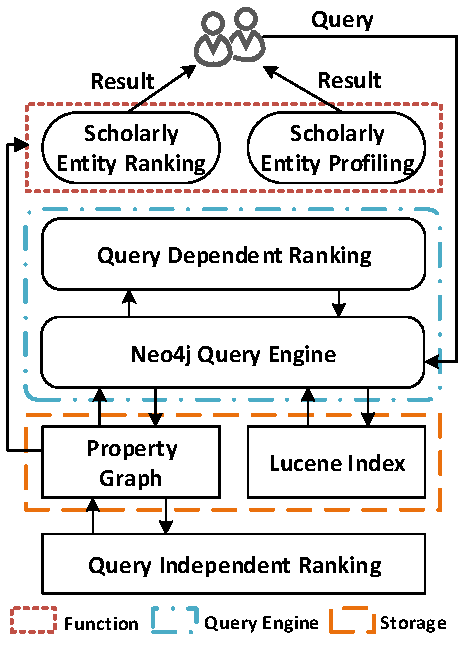
\includegraphics[width=0.9\columnwidth]{systemFrame.pdf}
\caption{System Framework}
\label{fig:frame}
\vspace{-2ex}
\end{figure}


\begin{figure}
\centering
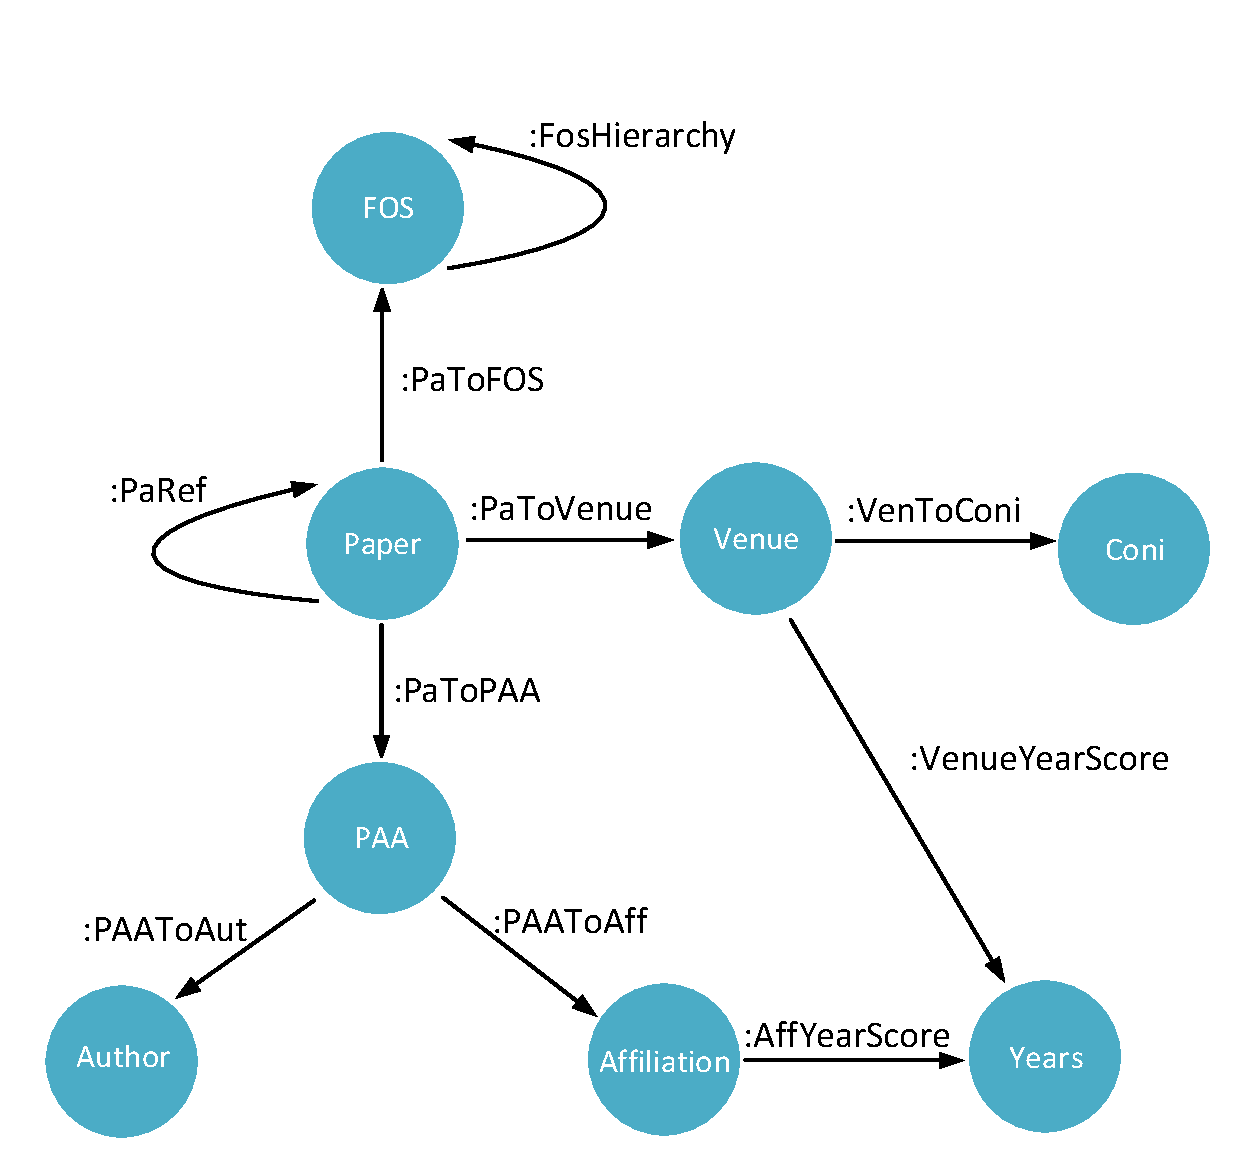
\includegraphics[width=0.5\columnwidth]{neo4jSchema.pdf}
\caption{Neo4j Schema Design}
\label{fig:schema}
\vspace{-3ex}
\end{figure}

\begin{figure*}[tp]
\centering
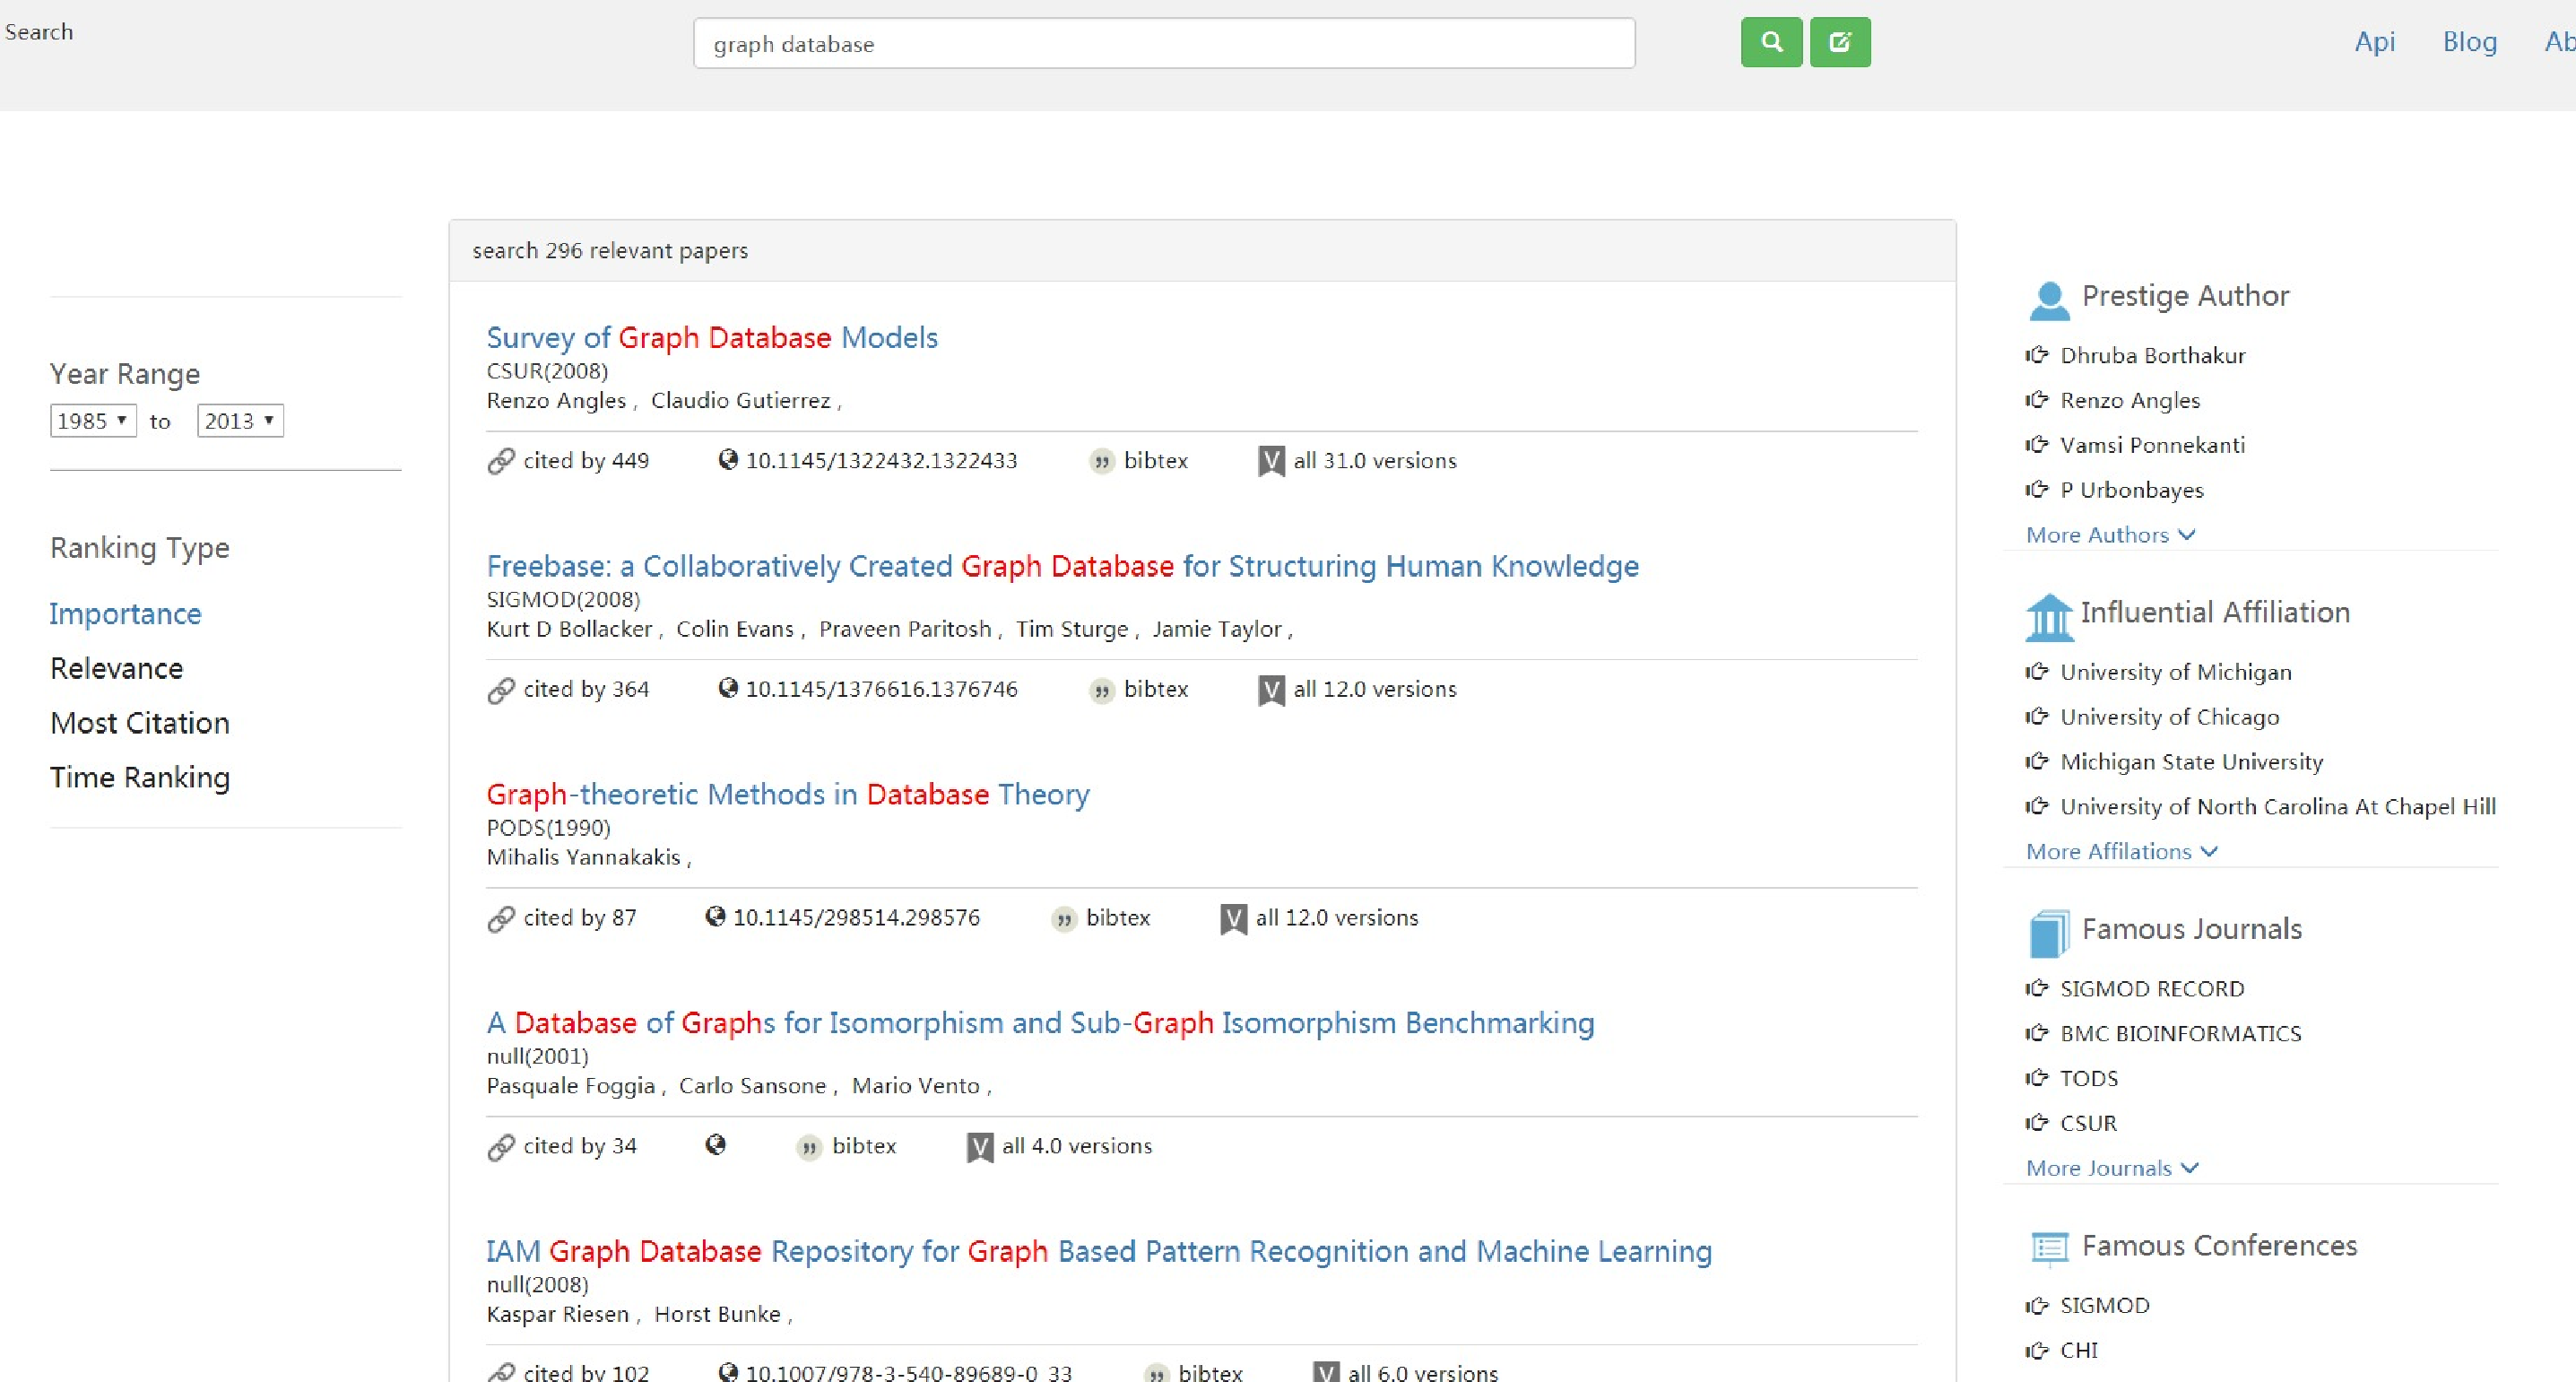
\includegraphics[width=\textwidth]{searchKeywords110.pdf}
\caption{Search Keywords And Heterogeneous Entity Ranking}
\label{fig: search keywords}
\vspace{-3ex}
\end{figure*}

\par
We mainly use Microsoft Academic Graph(MAG) to build \oursystem ~\cite{sinha2015overview}. It contains about 126 million scientific publication records, 529 million citation relationship and other scholarly activities information. Fig. \ref{fig:frame} shows the framework of our system, which consists of three main components, \emph{Storage, Query Engine} and \emph{Visualizer} respectively. Based on the framework, we then present a set of web-based scenarios using RESTful APIs.
% 126909021 paper  114698044 articles 529 million

\subsection{System Framework}
%Data source. currently storage solution, shortage, why graph database. storage contents

\subsubsection{Storage}
%We mainly use Microsoft Academic Graph(MAG) to build \oursystem \cite{sinha2015overview}. It contains scholarly information such as author, article, venue, affiliation, field of study as well as other information. Aminer, CiteSeerx and Semantic Scholar use relational database system such as Mysql to store and manage the xxx.

Scholarly data highly connected by reference relationship between articles and constructs a huge heterogeneous graph. Aminer, CiterSeerx and Semantic Scholar use RDBMS such as Mysql to store and manage scholarly data. While Acemap apply Spark to operate massive memory data and Microsoft Academic use Azure to store those huge data. Take RDBMS as an example, complex joins and self-joins will incur obviously performance bottleneck when the scholarly dataset becomes more inter-related. A comparison of the performance of querying the cited articles of an article using RDBMS(Mysql) and graph database(Neo4j) is given in table 1. Furthermore, our heterogeneous entities ranking algorithm, a type of Time-Weighted PageRank bases on graph structure, assesses the importance of nodes in a heterogeneous graph. Thus, it utilizes a popular graph database Neo4j to store and manage heterogeneous scholarly data.
% scholarly data source, currently solution, why graph database.

\par
The component of storage consists of property graph and transaction. Heterogeneous academic data is stored as property graph model which possesses nodes and relationships, and we use transaction to ensure the predictability of relationship-based queries.
% storage

\par
In order to retrieve and rank heterogeneous scholarly entity efficiently, we design the Neo4j graph schema mainly based on two principles. (1) Nodes for things and relationships for structure. (2) Reduce fine-grained relationship names while increase generic relationships qualified with property appropriately. Thus, we model scholarly data as a huge heterogeneous graph, shown in Fig. \ref{fig:schema}, which contains more than one billion nodes and over two billion relationships.
% design principles and schema.
% We take into consideration of the query ability of the graph schema and adopt specific time and space trade-offs. heterogeneous scholarly entity ranking ?

\par
The graph schema contains seven type of entities: author, affiliation, field of study, paper, venue(journal and conferences \eg KDD, ICDE ), conference instance (\eg KDD 2019, ICDE 2019), years. In order to query efficiently(?), we introduce an additional node PAA to represent the paper-author-affiliation n-ary relationships. Intuitively, a paper get published in a journal/conference by the author means new edges among paper, author and venue node. By employing ranking model as stated in section \ref{sec-model}, we derive affiliation, author, venue and article ranking score using incremental computation \cite{ma2018query}. And those score is described as a property in the graph schema.
% explain our schema

%In fact, we can apply any other ranking algorithms to rank scholarly entities in the graph schema.


\subsubsection{Query Engine}
\oursystem supports a variety of queries on scholarly graph that involves keywords retrieval, subgraph search, top-k important heterogeneous entities. Query engine is the main component that is responsible for a common set of queries from graph database. It consists of Lucene index, query optimization, Neo4j query engine and ranking algorithm.
% add heterogenous entity Ranking ?

\par
\oursystem takes the advantage of Lucene index that is an inverted index. For the purpose of query efficiently, we employ Lucene index in property of paper title, author name and distributed representation of words. Query optimization aims to reduce cardinality of work in the progress to generate a new query plan, such as hitting index, reducing matching paths. Moreover, Neo4j query engine executes the query plan to perform efficient data retrieval. And search results are aggregated by SARank, relevance, citation, year, average and maximum functions.
% query engine; function(?)

\subsubsection{Visualizer}
With all the technical details of managing and querying scholarly data in the system back-end, the ranking system takes users queries through user interfaces, dispatches them to the query engine, and receives the answers back to visualize. The next subsection presents some scenarios to demonstrate the front-end.

\begin{figure}
\centering
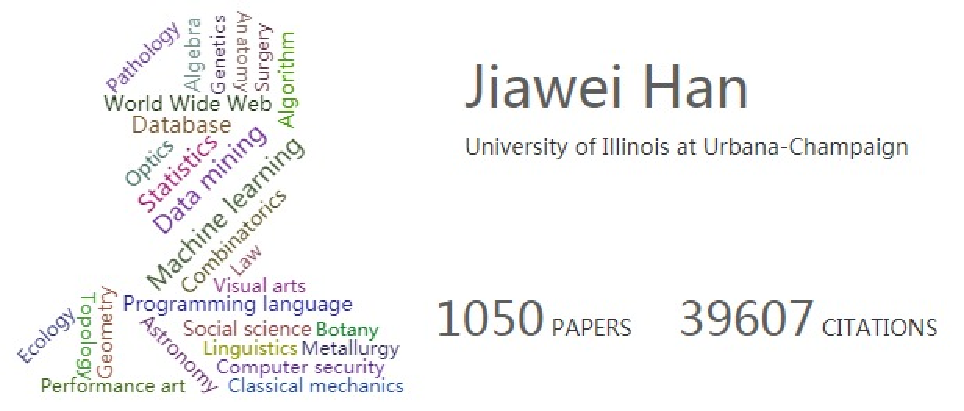
\includegraphics[width=\columnwidth]{hjwAvatar.pdf}
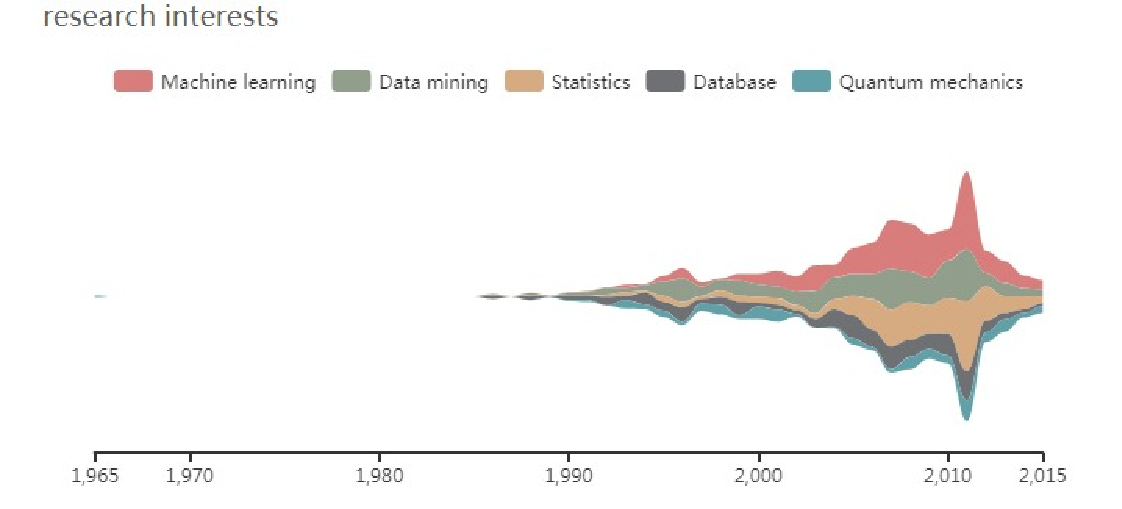
\includegraphics[width=\columnwidth]{hjwInterest.pdf}
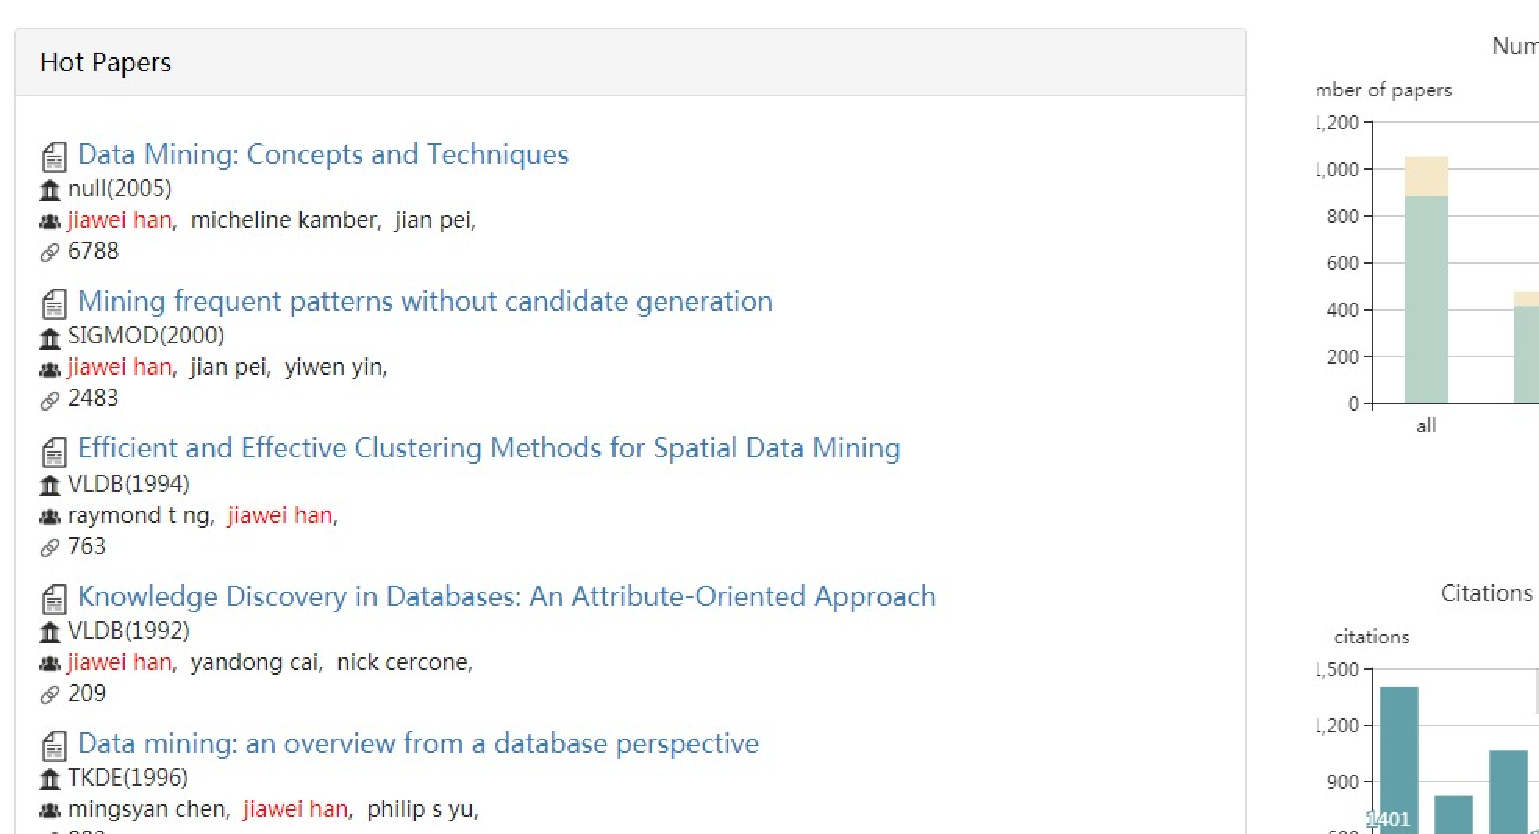
\includegraphics[width=\columnwidth]{hjwPapers.pdf}
\caption{Author Profiling}
\label{fig:hjwProfile}
\vspace{-3ex}
\end{figure}



\subsection{System Demonstration}
\par The demonstration consists of three parts. (1) we demonstrate its ranking models and heterogenous entity rankings given the query keywords by \oursystem. (2) To further illustrate the effective ranking model based on importance, we take {\em time ranking} in SIGMOD as an example. (3) We also demonstrate author profiling for a better knowledge of the author.


\stitle{Article Ranking and Keywords Profiling}. Fig. \ref{fig: search keywords} is an example of Search Page. In this page, we fulfill the query need with their ranking metrics and construct keywords profiling,
try to answer which authors/venues/affiliations are the most authoritative in the queried field of study.

\par

It has four major areas: (1) Area 1, the top of the picture, where users can search keywords, authors, affiliations, journal and conference (2) Area 2 presents influential papers about the keywords and {\em relevance} for default ranking metric, which is in the center of the picture. (3) At left of the picture is Area 3, users can specify different ranking metrics such as {\em relevance}, {\em importance}, {\em citation}, {\em year} to fit various ranking scenarios. (4) Top-k prestige authors, influential affiliations, famous journals/conferences corresponding to ranking metrics and keywords are shown in Area 4, which is at the right of the picture.

% keywords search and profiling.

\stitle{Ranking Instance}


\begin{figure}
\centering
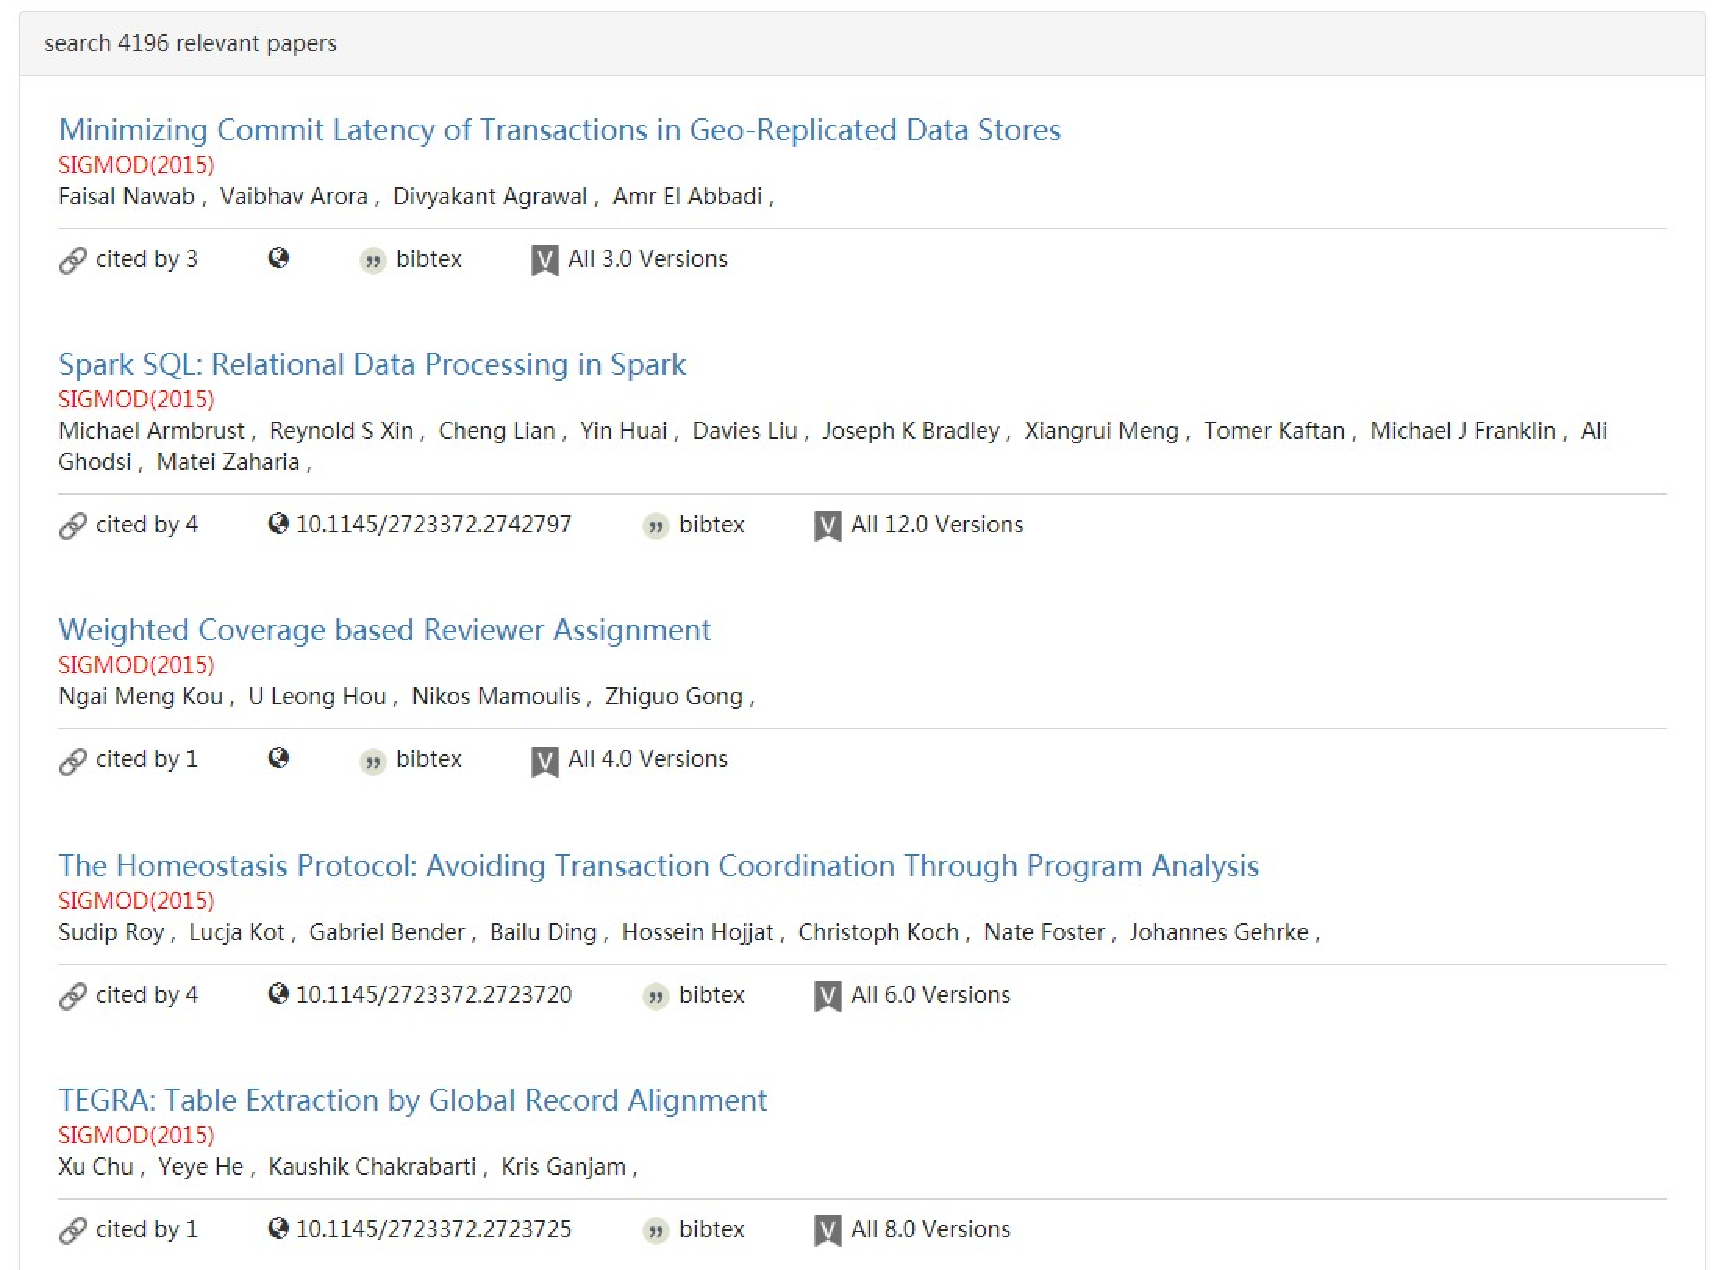
\includegraphics[width=\columnwidth]{sigmod15.pdf}
\caption{SIGMOD 2015}
\label{fig:sigmod}
\vspace{-3ex}
\end{figure}


\stitle{Author profiling}. Fig. \ref{fig:hjwProfile} is an example of an Author Page, where contains author's basic information and author's detailed profiling. For basic information, users can check author's publications, related authors and author's affiliations. We also develop author's detailed profiling to have a knowledge of the author both from breadth and depth. Thus, we model the evolution of author's research interest, author's avatar with word cloud description, the statistics of publication, {\em etc}.
%author profiling


%\par
%\stitle{Affiliation profiling}. As shown in fig. \ref{}, we give an example of affiliation profiling. The layout of the Affiliation Page is similar with Search Page, users can discover publications using various ranking metrics and check statistics information, such as the importance author, relevant affiliation, famous journals/conferences.
%% affiliation profiling

%\par
%\stitle{Venue profiling} venue
